\documentclass[12pt]{article}
\usepackage{graphicx}
\usepackage{enumitem}
\usepackage{amsmath}
\usepackage{gvv-book}
\usepackage{gvv}

\title{\textbf{System of Equations}}
\author{\textbf{EE25BTECH11008 - Anirudh M Abhilash}}
\date{October 4, 2025}

\begin{document}

\maketitle

\section*{Question}

Solve the following system of equations:
\begin{align*}
x - y = 8, \\ 3x - 3y = 16
\end{align*}

\section*{Solution}

Each equation can be expressed in vector form as a dot product:
\begin{align}
\myvec{1 & -1}\myvec{x \\ y} &= 8, \\
\myvec{3 & -3}\myvec{x \\ y} &= 16.
\end{align}

Stacking these gives the matrix equation
\begin{align}
\myvec{1 & -1 \\ 3 & -3}\myvec{x \\ y} &= \myvec{8 \\ 16}.
\end{align}

In augmented form,
\begin{align}
\augvec{2}{1}{1 & -1 & 8 \\ 3 & -3 & 16}.
\end{align}

Applying the row operation $R_2 \to R_2 - 3R_1$,
\begin{align}
\augvec{2}{1}{1 & -1 & 8 \\ 0 & 0 & -8}.
\end{align}

This yields the contradiction
\begin{align}
0 = -8.
\end{align}

Hence the system is inconsistent,
\[
\boxed{\text{No solution}}
\]

\begin{figure}[H]\centering
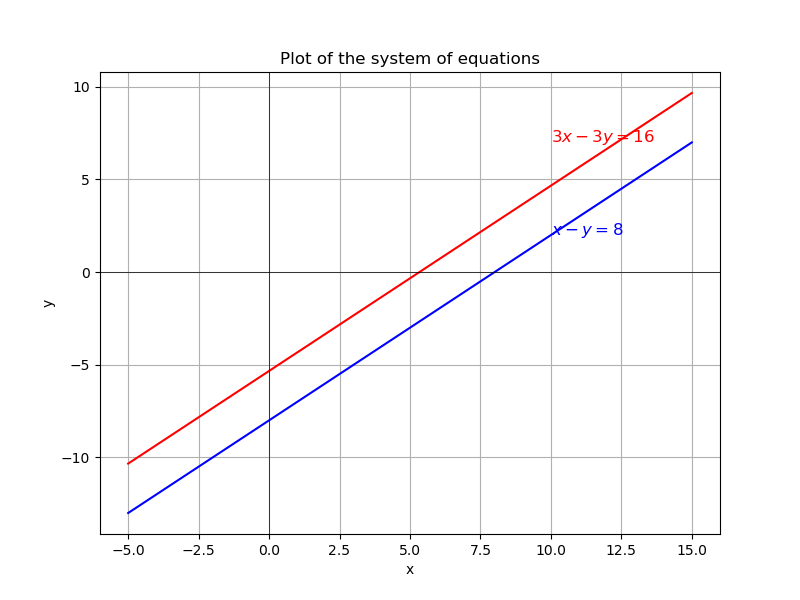
\includegraphics[width=1\columnwidth]{figs/plt.png}
\caption{Lines}
\label{fig:plt}
\end{figure}


\end{document}
